\documentclass[11pt, a4paper]{article}

\usepackage[utf8]{inputenc}

\usepackage[colorlinks=true,urlcolor=magenta]{hyperref} %Used for hyperlinks to reference materials, and section referencing.
\usepackage{tabulary} %used for tables.
\usepackage{booktabs} %Used for nicer table formatting eg midrule
\usepackage{graphicx} %Used for, well, graphics
\usepackage{float} %Used to put graphics in their place
\usepackage{enumitem} %Used for modifing the labels used for items in lists. http://mirror.ox.ac.uk/sites/ctan.org/macros/latex/contrib/enumitem/enumitem.pdf
\usepackage{rotating} %Used for sideways figures


\usepackage{pdflscape}%Allows pages to be made landscape in conforming PDF viewers.Unknown behaviour when printing.
%http://mirror.ox.ac.uk/sites/ctan.org/macros/latex/contrib/oberdiek/pdflscape.pdf

\def\sectionautorefname{Section}
\def\subsectionautorefname{Subsection} % Reassigning the default names to have capitals.
%The command gives hyperlinked referencings in the form Section #: SectionTitle
\newcommand{\gref}[1]{\hyperref[#1]{\autoref*{#1}: \nameref{#1}}} % Good referencing = gref

\def\itempar#1\\{\item \textbf{#1}\\} %Macro to automatically bold the first line of an item in a list. Usage is \itempar Line1\\ Line 2...Line N

\def\textul#1{\underline{\smash{#1}}} %Proper text underlining, where the line is not a mile away from the text

\begin{document}

\begin{titlepage}
	\thispagestyle{empty}
	{\centering
		
\includegraphics[width=0.5\textwidth]{heriot-watt-logo.png}\par\vspace{1cm}
	%	{\scshape\LARGE Heriot-Watt University \par}
		\vspace{1cm}
		{\LARGE F21DG - Design and Code Project\par}
		{\LARGE \par}
		\vspace{1.5cm}
		{\scshape\Large MACS Department Workload Management System\par}
		\vspace{1.5cm}
		{\scshape\LARGE\bfseries Project Report \par}

		\vspace{3.5cm}
			\begin{center}
					April 23\textsuperscript{rd} 2020
			\end{center}
		\textit{Authors}\par
		\begin{tabular}{rcl}
			\\ \textsc{Tommy Lamb} & - & H00217505\\
			\textsc{Dylan Forrest} & - & H00216546\\
		\end{tabular} \\
	
	}
\end{titlepage}

\section{Context and Scope}

As per the earlier requirements specification document, this project was to implement a workload management system for the MACS department. As we were developing from a substantial existing system, which was non-functional, we decided to limit our initial scope to restoring functionality and laying the bedrock for future expansion. Our intention as the project progressed was to expand this scope to introduce the new features identified in the functional requirements.

To provide for future feature development we included the redesign and implementation of the supporting database (TODO link to section) as part of this initial target. Our motivation for this was two-fold. Firstly the database is the most important component with regards to implementing many of the new features, and secondly, its design could have significant ramifications on other components’ implementation and design. We felt it would be counterproductive to repair the system to work with the existing database only to later replace it entirely, especially as we were uncertain how much work would be required to restore functionality.

As the project progressed we were unable to expand our scope beyond this as we had hoped. For further details we direct the reader to (TODO link this) the evaluation section.


\section{Database design}

From the outset it was quickly apparent that the existing database implementation was deficient and would require a significant redesign and implementation. The most glaring issue was the lack of any foreign-key constraints on the data. In defence of the previous developers we suspect this was down to technical limitations of the storage engines available in MySQL at the time. Possibly motivated by this so as to avoid table joins, there was also some amount of data duplication inherent in the schema. This, combined with the need to add new columns and tables to hold the data for new functionality, led us to implement our database from a largely clean slate, but with obvious reference to the previous schema.
\begin{landscape}
	\begin{figure}
	\thispagestyle{empty}
		\centering
		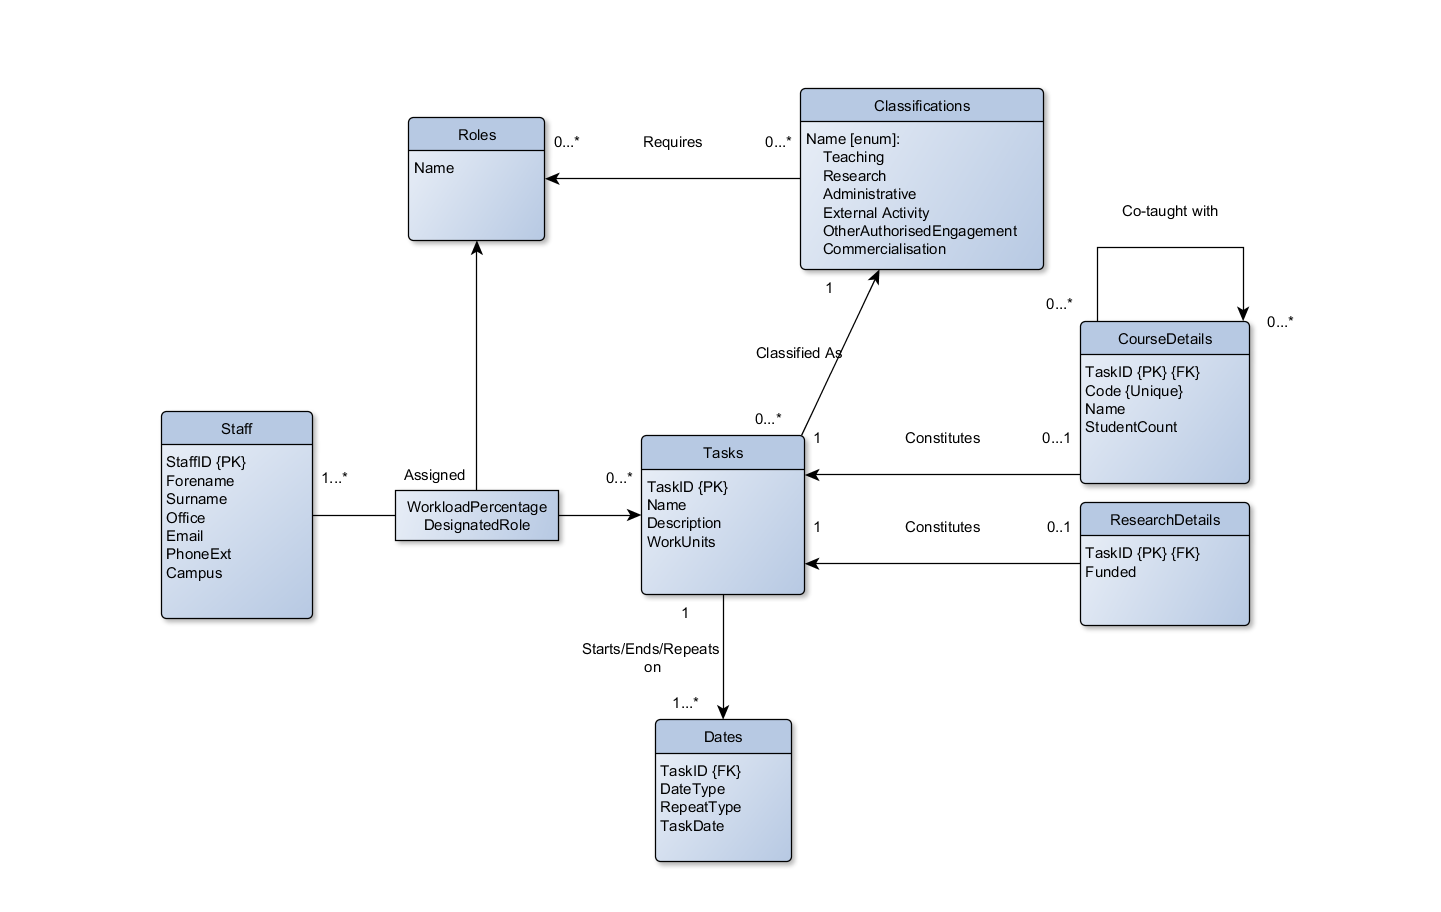
\includegraphics[scale=0.45]{DatabaseDiagram.png}
		\caption{ER diagram for the database}
	\end{figure}
\end{landscape}

The schema we devised is shown in figure 1, with individual tables and relations discussed in relevant sections below:

\subsection{Staff}
Expanding on the original database, we now store contact details for a staff member. Ideally these would be read from an existing database in the department, but we don’t know if any such database exists. This could be changed in future with relative ease. Note that we do not store any login details here, such as a password hash, due to our intention to use LDAP. Currently we use the existing login accounts table from the previous DB, as this was completely disjoint from the rest of the database anyway.

The office field is intended to match Heriot-Watt’s standard naming convention: for example, EMG44 would refer to Earl Mountbatten building, Ground floor, room 44.

\subsection{Tasks}
The tasks table holds details common to all different task types, with task-type-specific details stored in separate tables. This was done to make it easier to provide aggregate and general-purpose queries across all task-types at the minor cost of making task-specific queries require a table join. In our estimation a greater number of queries being made to the DB would be agnostic to the extra details than those that require them, making this a worthwhile trade-off.

WorkUnits here is an abstract numerical representation of the total amount of work required by the task. The exact nature of these values is left to be defined at the organisational level, whether they be relative values or absolute values based on some metric (such as time requirements). WorkUnits is intended to be independent of the staff members assigned to the task.

\subsection{Classifications and Roles}
The classifications table is simply to allow the conceptual grouping of tasks within the system. An important requirement was to see the division of staff members’ time between the various types of tasks they perform. This table also enables the system at the application layer to better handle the abstraction of the Tasks, ResearchDetails, and CourseDetails tables.

Certain types of tasks, such as Research tasks, have specific roles associated (and sometimes required) by them. In the case of research, each task must have a Principal Investigator assigned. Since MySQL does not properly support business constraints of this nature, this must be enforced at the application layer. The relation between the roles and classifications table is designed to facilitate this in a scalable and easily adaptable manner. Note that some entries in the Roles table are entirely optional.

\subsection{Dates}
The previous DB utilised a rigid date system that used the academic semesters and holidays between them as single blocks. To improve the granularity and usefulness of data we decided to move to using full dates, as tasks may well start and end partway through a semester. In addition to this we wanted to support tasks that were indefinite and those that had a defined period, but repeated each year/semester etc. As there was an expressed desire to use the academic date system, we decided to use the standard calendar system for underlying storage due to better support and reduced complexity. We planned to perform on-the-fly translation between the two systems in the application layer in order to support the academic calendar.

DateType here is a numerical value intended to be used by the application to distinguish between different date types, such as Start and end dates, and single day events.

RepeatType is also a numerical value intended to specify how a date repeats, for example, annually, per semester, never, etc.

Both DateType and RepeatType values only have meaning to the application layer, and so their precise values are left for it to define.

TaskDate is the date field used to hold the date itself. The name was chosen since DATE is a reserved word in SQL.

\subsection{Relation on Staff, Tasks, and Roles}

This relation captures the assignment of staff members to particular tasks, and the details of that assignment. In particular: if that staff member fulfills any particular named role within that task, hence the relation to the Roles table, and what percentage of the task they contribute to. Constraints and requirements on these values are defined in the Requirements Specification document.

\section{Development}

\subsection{Automated Testing}

Currently there are no auto-tests as we ran out of time to create them but the testing environment is setup and ready to run auto tests.
We are using codeception which is a PHP testing framework that features the ability to run unit, functional and acceptance tests on the website. Once anything is pushed to the github repository Travis CI (our continuous integration) will run each test found in the tests folder and either pass or fail the build depending on the outcome of the tests.


\subsection{Configuring a Development Environment}

\subsubsection{Prerequisites}
LAMP stack installed on development/live server. A guide to installing a LAMP server environment can be found here:\\ \href{https://www.digitalocean.com/community/tutorials/how-to-install-linux-apache-mysql-php-lamp-stack-ubuntu-18-04}{https://www.digitalocean.com/community/tutorials/how-to-install-linux-apache-mysql-php-lamp-stack-ubuntu-18-04}

\begin{itemize}
\item PHP Version \textgreater= 7.0
\item MySQL Version \textgreater= 5.7
\item Apache2 \textgreater= 2.4
\end{itemize}

\subsubsection{Installation}
Place the \texttt{src/} folder into your \texttt{public\_html} folder.

\subsubsection{Setting up MySQL database}

\begin{enumerate}
\item Create empty database called ‘csm’\\
\texttt{mysql> CREATE DATABASE csm;}

\item Import \texttt{sql/CreateDatabase.sql} to the new ‘csm’ database.\\
\texttt{shell> mysql -u <username> -p csm < CreateDatabase.sql}

\item \texttt{src/php/core/mysql.php} line 26: update each of the parameters so they match the database you wish to connect to.\\
 \textbf{Note:} We plan to change this in the future as this way isn’t secure.
 
 \item 	(Optional) Import \texttt{sql/InsertData.sql} to the ‘csm’ database to import test data.\\
 \texttt{shell> mysql -u <username> -p csm < InsertData.sql}
 
 \item (Optional) If you loaded in the test data there is a test username and password provided:\\
username: test\\
 password: qwerty
\end{enumerate}


\end{document}